\documentclass[11pt]{article}


%% ----------------------------------


\usepackage[margin=1in]{geometry}

% use proper unicode fonts
\usepackage[T1]{fontenc}
\usepackage[utf8]{inputenc}

\setlength{\parindent}{0pt} % remove automatic indent

\usepackage{amsmath} % for better display of equations

\usepackage{natbib} 

%% ----------title ------------------------

\usepackage{titling} % controls the way the title information is displayed
\pretitle{\begin{flushleft}\Large}
\posttitle{\end{flushleft}}
\predate{}
\postdate{}
\preauthor{\begin{flushleft}}
\postauthor{\end{flushleft}}
\setlength{\droptitle}{-3em}

\usepackage{authblk} % adds some nice options for displaying the author list

%---------------- plots -----------

\usepackage{pgfplots}
\usepackage{pgfplotstable}
\usepackage{tikz}
\usepackage{tikz-cd}
\usetikzlibrary{calc, shapes}
\usetikzlibrary{shapes.geometric,shapes.arrows,decorations.pathmorphing}
\usetikzlibrary{matrix,chains,scopes,positioning,arrows,fit}
\tikzstyle{every picture}+=[remember picture]

\usepackage{graphicx}
\usepackage{float}
\usepackage{sidecap}
\sidecaptionvpos{figure}{c}
\usepackage{wrapfig}
\usepackage[font=scriptsize]{caption}
\graphicspath{{tex/}}

%% ---------comments-------------------------

\usepackage{comment}
% 1- specify a new environment
% 2- use includecomment{} makes it appears in the pdf without format distinction (useful for edits)
% 3- use excludecomment{} makes it invisible in the pdf (useful for comments)
% available colors: red, green, blue, cyan, magenta, yellow, black, gray, white, darkgray, lightgray, brown, lime, olive, orange, pink, purple, teal, violet
\specialcomment{IB}{\begingroup\sffamily\color{blue}\footnotesize\flushleft\textsuperscript{IB}}{\endgroup} % comments
\specialcomment{DG}{\begingroup\sffamily\color{olive}\footnotesize\flushleft\textsuperscript{DG}}{\endgroup} % comments
\specialcomment{TD}{\begingroup\sffamily\color{red}\footnotesize\flushleft\textsuperscript{TD}}{\endgroup} % comments

% use as \begin{IB} ... \end{IB}

\usepackage[normalem]{ulem} % for strikeouts using \sout{}
\usepackage[textsize=footnotesize, backgroundcolor=white]{todonotes} % for margin notes using \todo{}


%% ----------------------------------
%
%     Title and authorship information
%
%% ----------------------------------


\title{How vegetation-herbivores feedbacks mediate the temperate-boreal forest transition?}
\date{}
\author[1]{Isabelle Boulangeat}
\author[2]{Mathieu Leblond}
\author[3]{Tanguy Daufresne}
\author[1]{Steve?, Matt?}
\author[1]{Dominique Gravel}
\affil[1]{Département de biologie, Université du Québec à Rimouski, 300, Allée des Ursulines, Rimouski, QC, G5L 3A1, Canada}
\affil[3]{INRA - UMR 210 Eco\&Sols - Bat 12, 2 Place Viala, F-34060 Montpellier cedex 1}



%% ----------------------------------
%
%     END PREAMBLE
%
%% ----------------------------------

\begin{document}

%% ----------------------------------
%
%     TITLE PAGE
%
%% ----------------------------------


\maketitle

% \begin{flushleft}
% \textbf{Keywords:} Uncertainty, scaling, range dynamics, trees, disturbances, patterns and processes, predict or understand, climate change, biotic interactions, spatial ecology, decision making, metamodelling, species distribution modeling
% \end{flushleft}


%% ----------------------------------
%
%     REST OF DOCUMENT
%
%% ----------------------------------


% \begin{IB}
% comment exemple
% \end{IB}

%% \begin{TD} pour Tanguy et \begin{DG} pour Dom

%% ************************************************************

%% Context

%% *************************************************************
\section{Contexte}

De nombreux travaux scientifiques attirent l'attention sur les impacts
potentiellements conséquents des changements climatiques sur la composition
des forêts, et plus particulièrement encore au niveau des écotones. La forêt
tempérée devrait migrer vers le nord, à la place de la forêt boréale, où le
climat lui sera favorable dans peu de temps. Cependant, d'autres facteurs sont
suceptibles de créer un décalage entre le moment où le climat devient
favorable et celui où la forêt tempérée va pouvoir s'installer réellement.
Parmi les différents facteurs qui peuvent être à l'origine d'un tel décalage,
nous pouvons citer la démographie, l'histoire biogéographique et la capacité
de dispersion des espèces, les régimes de perturbations (\textit{e.g.,} les
feux), ainsi que les interactions biotiques (intra et inter niveaux
trophiques).

\vspace{1em}

\noindent A l'aide d'une approche de modélisation spatiallement implicite, nous nous
intéressons ici à caractériser, le long d'un gradient climatique, les
équilibres possibles entre la distribution de la végétation (forêt tempérée et
boréale) et les populations d'ongulés (cerf de virginie et orignal) en
interaction. L'originalité de ce travail est de s'intéresser à la transition
entre deux types de forêts, et de prendre en compte l'effet du climat et les
interactions trophiques via la relation consommateur-ressource qui traduit à
la fois l'impact des ongulés sur la végétation et celui de la végétation sur
les ongulés.


%% ************************************************************

%% Questions

%% *************************************************************

% \subsection*{Question générale}



%% ************************************************************

%% MODEL

%% *************************************************************
\newpage
\section{Model with two forest types}

In this case the forest is divided into three types $B$, $T$, and $M$ for
boreal vs temperate forest, and mixed stands. A fourth state is the
regeneration state, post disturbance $R$.

\vspace{2em}
\begin{center}
\begin{tikzpicture}
\matrix(m) [matrix of nodes, column sep=6em,
	row sep=4em,
	minimum width=4em,
	minimum height=4em,
	nodes={draw, circle, anchor=base}]
	{
	& T & \\
	R & & M \\
	& B & \\
	}; %end matrix

\draw[-angle 45] (m-2-1.north) to[bend left=10] 
node[midway,above, sloped] {$\alpha_T(M+T)[1-\alpha_B(M+B)]$} (m-1-2.170) ;
\draw[-angle 45] (m-1-2.west) to[bend left=10] 
node[midway,below, sloped] {$\epsilon_T$} (m-2-1.80) ;

\draw[-angle 45] (m-2-1.south) to[bend right=10] 
node[midway,below, sloped] {$\alpha_B(M+B)[1-\alpha_T(M+T)]$} (m-3-2.190) ;
\draw[-angle 45] (m-3-2.west) to[bend right=10] 
node[midway,above, sloped] {$\epsilon_B$} (m-2-1.280) ;

\draw[-angle 45] (m-2-1.10) to[bend left=5] 
node[midway,above] {$\alpha_T(M+T)\alpha_B(M+B)$} (m-2-3.170) ;
\draw[-angle 45] (m-2-3.190) to[bend left=5] 
node[midway,below] {$\epsilon_M$} (m-2-1.350) ;

\draw[-angle 45] (m-1-2.10) to[bend left=10] 
node[midway,above, sloped] {$\beta_B(B+M)$} (m-2-3.north) ;
\draw[-angle 45] (m-2-3.100) to[bend left=10] 
node[midway,below, sloped] {$\theta_T$} (m-1-2.east) ;

\draw[-angle 45] (m-3-2.350) to[bend right=10] 
node[midway,below, sloped] {$\beta_T(T+M)$} (m-2-3.south) ;
\draw[-angle 45] (m-2-3.260) to[bend right=10] 
node[midway,above, sloped] {$\theta_B$} (m-3-2.east) ;

\end{tikzpicture}
\end{center}

\vspace{1em}

\fbox{
\begin{minipage}{\textwidth}
$\alpha_B$, $\alpha_T$ are regeneration probabilities (related to seedling survival)

$\beta_T$ and $\beta_B$ are colonisation probabilities 

$\theta_T$ and $\theta_B$ are competitive exclusion probabilities in mixed forests
\end{minipage}
}

\subsection*{Species and states}

\begin{description}
\item[Regeneration: ] Bouleau jaune, Bouleau blanc (à papier), Chêne rouge, Peuplier baumier, Peuplier à grandes dents, Peuplier faux tremble, Pin blanc, Pin rouge, Cerisier de Pennsylvanie, Saule, Sorbier d'Amérique
\item[Boreal: ] Épinette noire, Épinette blanche, Épinette rouge, Thuya occidental, Mélèze laricin, Pin gris, Sapin baumier
\item[Temperate: ] Érable rouge, Érable à sucre, Frêne d'Amérique, Frêne noir, Hêtre à grandes feuilles, Ostryer de Virginie, Tilleul d'Amérique, Cerisier tardif, Pruche de l'Est
\end{description}

%% ************************************************************

%% Herbivore 

%% *************************************************************
\newpage
\section{Herbivores' dynamics}

Based on metaphysiological model \cite{Owen-Smith2002}

The herbivore dynamic will be modelled as a total biomass in the considered
landscape (AND NOT a number!)

%-----
\[
\left.
\begin{array}{r c l}{}

\frac{1}{H}\frac{dH}{dt} &=& 
\overbrace{(1-m)}^\text{annual survival rate}
(\overbrace{cI}^\text{biomass gains} - \overbrace{(p+e^{-zcI})}^\text{biomass losses})
- \overbrace{m}^\text{mortality by senescence, accidents, hunting...}

\end{array}
\right.
\]

\texttt{When $\text{losses}\geq (1+\text{gains})$ $\frac{dH}{dt}=-H$}

%-----

\vspace{1em}
\fbox{
\begin{minipage}{\textwidth}
$p$ is the metabolic attrition rate (per herbivore biomass unit)

$z$ is a decreasing parameter of mortality rate in function of intake

$m$ is the minimum mortality rate when food is abundant (senescence, accidents, hunting...)

$c$ is the conversion between ingested biomass and converted biomass

$I$ is the vegetation intake rate (consummed biomass per herbivore biomass unit - see next section for details)
\end{minipage}
}
\vspace{1em}


% Gains=losses=$I_K$ when:

% \[
% I_K = \frac{1}{cz}(pz + LambertW(ze^{-pz}))
% \]


\begin{SCfigure}[0.9][h]
\centering
   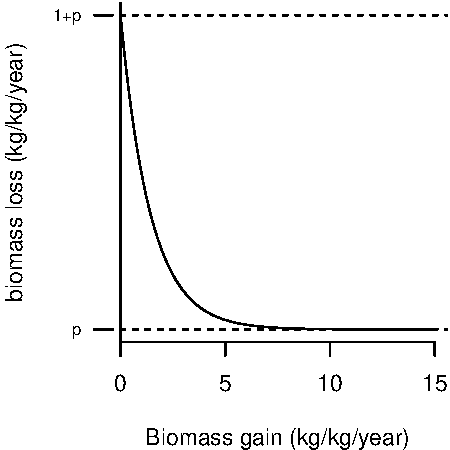
\includegraphics[width=0.5\textwidth]{../graphs/herbivore_mortality.pdf}

   \caption{Herbivore mortality depends on the intake. The figure illustrates
   this relationship for p = 5.84; z = 1}

\label{herbiMort} 
\end{SCfigure}


\newpage
\section{Interactions}
%% ************************************************************

%% resources intakes 

%% *************************************************************

\subsection{Resources intakes}

The intake (biomass consumption per herbivore biomass per time unit) will
depend on available resource and the herbivore preferences to have the best
quality food. Let's $R_1$ be the available preferred resource and $R_2$ the
available secondary resource (per herbivore biomass unit). The intake from
$R_2$ will depend on the relationship between the intake from $R_1$ and $p+m$
(minimum biomass loss rate).

\[
I = \overbrace{\frac{\tau F}{\mu+F}}^\text{intake rate of preferred resource} 
+ \overbrace{\frac{\rho G}{\nu+G}\Big(\phi + \frac{1-\phi}{ 1+e^{r(\frac{\tau F}{\mu+F} - p)}}}^\text{intake rate of secondary resource} \Big)
\]

\fbox{
\begin{minipage}{\textwidth}
$\tau$ and $\rho$ is are the maximum rates of intake (vegetation biomass per
herbivore biomass per year) Should be >$p$ for allowing herbivore positive growth.

$\mu$ and $\nu$ are half saturation parameter for resource intake (available
resource for which the intake is half) have to be >= $\tau$ ($\tau$ (or $\rho$)/(search rate))

$\phi$ is the coefficient of use of secondry resource when primary resource is abundant. It
might be greater than zero in order to depict winter forage and the time spent
in forest patches for protection reasons, and consequently a mimimum use as a
resource too.

$r$ is a smoothing parameter for the swich between use/non-use of the non-
preferred resource.
\end{minipage}
}


\begin{SCfigure}[1][h]
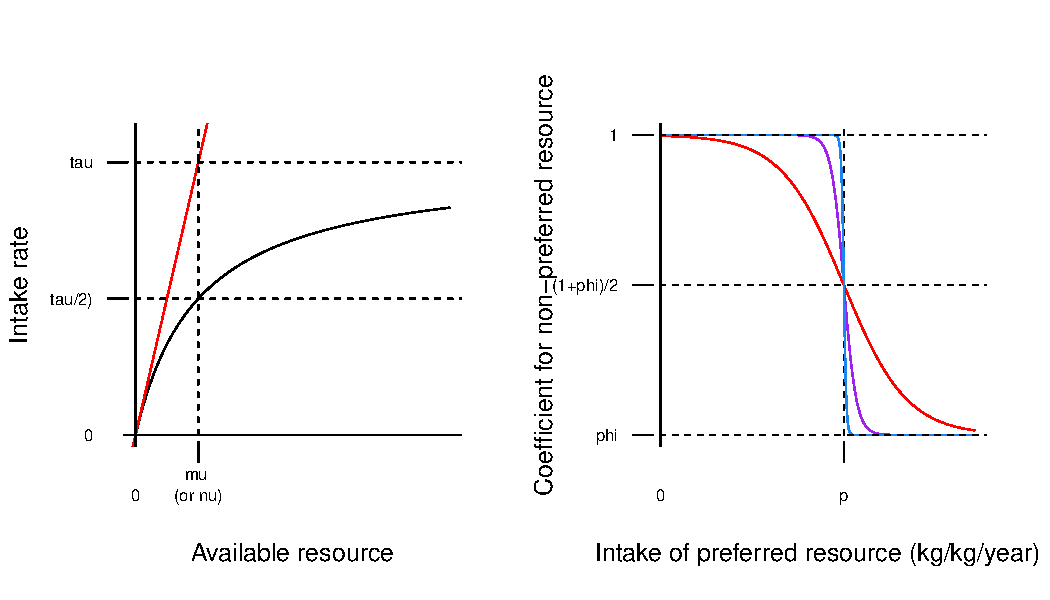
\includegraphics[width=0.7\textwidth]{../graphs/intakes.pdf}
   
   \caption{Use of resources. The figure illustrates the mechanisms for $\tau$ = 10; $\mu$ = 10; p = 5.84; z = 1; $\phi=0.8$; r = 1 (red); r = 5 (purple); r = 25 (blue)}
\label{resources}
\end{SCfigure}

\newpage
\subsubsection*{Two herbivores: Moose $H_a$ and White-tail deer $H_v$}

Preferred resources 
\[
\boxed{
F_a = ukR/H_a
}
\]
\[
\boxed{
F_v = u(1-k)R/H_v
}
\]

Secondary resource 
\[
\boxed{
G_a=(vT + wB + xM)k/H_a}
\]
\[
\boxed{
G_v = (vT + wB + xM)(1-k)/H_v
}
\]

\fbox{
\begin{minipage}{\textwidth}
$u$, $v$, $w$ and $x$ are conversions between areas and available biomass (i.e., vegetation density, accessibility), and $k$ is the competitive ability of $H_a$ on $H_v$.
\end{minipage}
}

\[
k = e^{-\ln(\frac{1}{k_0})\frac{H_v}{H_a}}
\]

In order to match these conditions:
\[
\left.
\begin{array}{l}
k = 1 \text{ if } H_a=0\\
k = 0 \text{ if } H_v=0\\
k = k_0 \text{ if } H_a=H_v
\end{array}
\right.
\]

$k_0=0.5$ will be used as parcimonious approach. The competitiveness therefore is only varying according to relative biomasses. 

\paragraph{Range of variation of total intake I}

$I_a \in$ [0; max($\tau_a k; \tau_a$)]
et
$I_v \in$ [0; max($\tau_v, \tau_v (1-k)$)]


\subsection*{Shelter effect}

The parameter $m$ might be dependent on $B$ (for Moose)

\[
m = \frac{m_s}{(1+(\frac{m_s}{m_0}-1)B)}
\]
\begin{SCfigure}[1][h!]
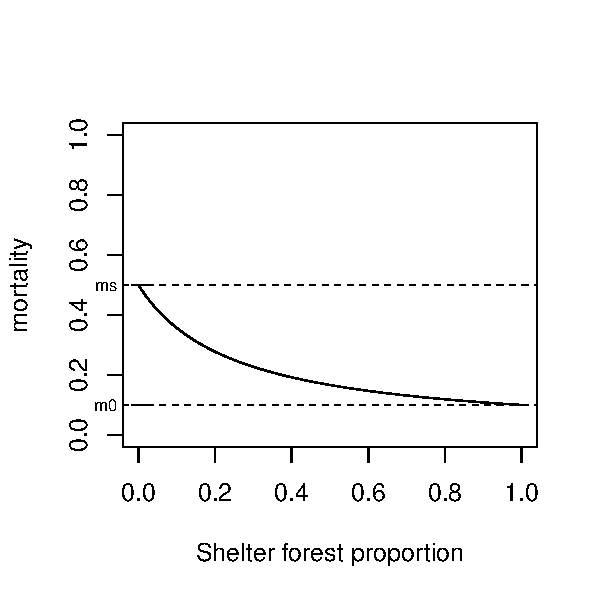
\includegraphics[width=0.4\textwidth]{../graphs/shelter_effect.pdf}
  \caption{Protective effect of the boreal forest for the moose. $m$ decreases with $B$. $m_0$ = 0.1; $m_s$ = 0.5 }
\label{shelter}
\end{SCfigure}

\fbox{
\begin{minipage}{\textwidth}
$m_0$ is the mortality (independent from resource) when B=1

$m_s$ is the mortality when B=0 (maximum predation and exposition to winds)
\end{minipage}
}

%% ************************************************************

%% herbivore coexistence

%% *************************************************************

\newpage
\section{Herbivores (co)existence}

For each herbivore alone, we can compute the biomass at equilibrium ($\frac{dH}{dt}=0$) for a given landscape ($R, T, B, M$ proportions).

\begin{SCfigure}[1][h]
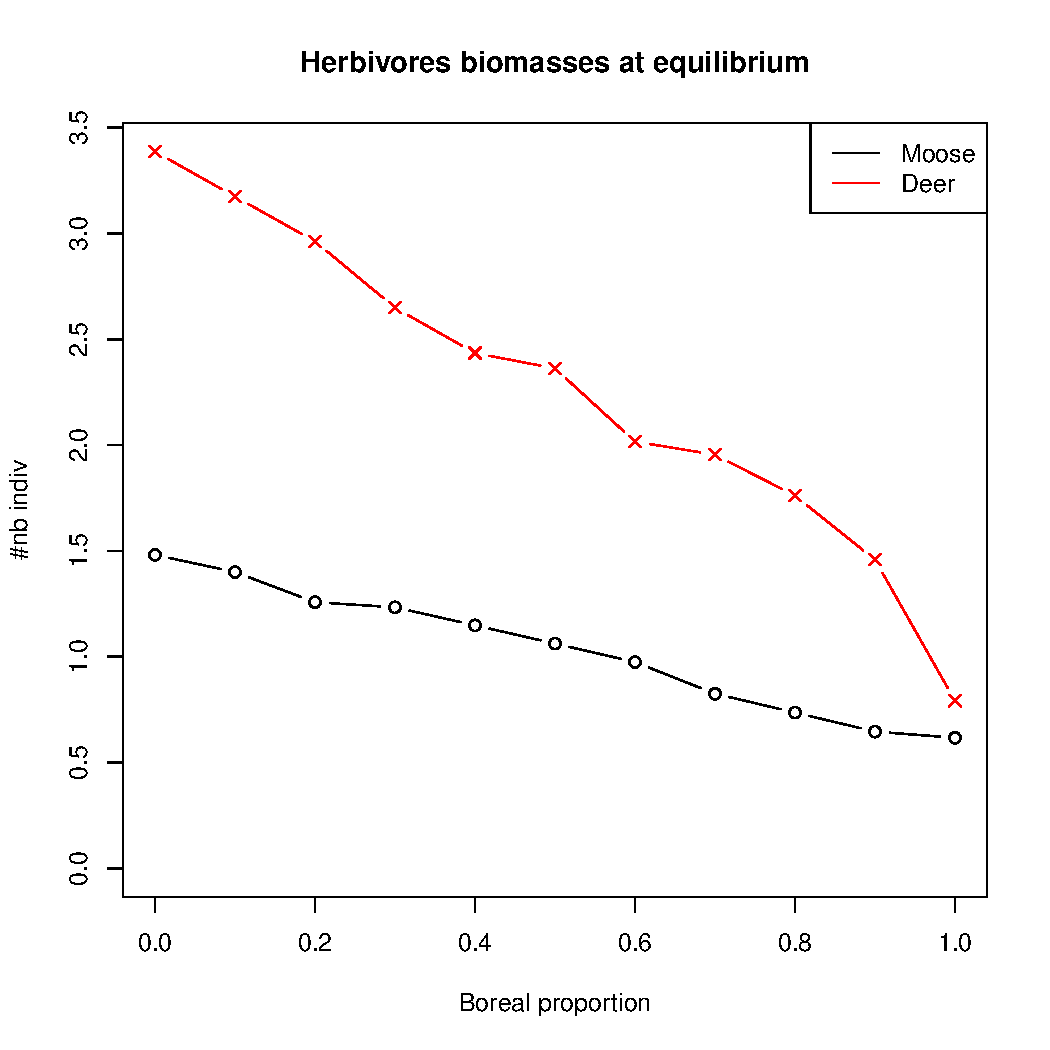
\includegraphics[width=0.7\textwidth]{../graphs/herbivore_eq_biomasses.pdf}
  \caption{Conditions of existence of the two types of herbivores. The maximum biomass per borel proportion is represented. In this exemple the parameters are (for 17ha) u = 17000; v=8700; w=3400; x = 5100; $p_a$ = 0.51; $z_a$ = 1; $c_a$ = 1; $m_{a_0}$ = 0.05; $m_{a_s}$ = 0.07; $\tau_a$ = 5.11; $\mu_a$ = 51.1; $\nu_a$ = 10.22; $\phi_a$ = 0.2; $r_a$ = 5; $p_v$ = 1.75; $z_v$ =1; $c_v$ = 1; $m_v$ = 0.2; $\tau_v$ = 8.75; $\mu_v$ = 87.5; $\nu_v$ = 17.5; $\phi_v$ = 0.2; $r_v$ = 5 }
\label{coexistenceH}
\end{SCfigure}





\newpage
%% ************************************************************

%% feedbacks on vegetation 

%% *************************************************************
\subsection{Feedback effects: impacts on the vegetation}

Based on the fact that the impact on demography is as much or more important
than the impact on biomass (\cite{Moncrieff2014}). The herbivores will affect
$\alpha$, $\beta$ and $\phi$ depending on the herbivore pressure on each
vegetation state.

\subsubsection*{Impact on R and $\alpha$}

Per biomass unit intakes for preferred resources (ie R):

\[
I_{a_1} = \frac{\tau_a F_a}{\mu_a+ F_a}
\]

\[
I_{v_1} = \frac{\tau_v F_v}{\mu_v+ F_v}
\]

\fbox{
\begin{minipage}{0.7\textwidth}
We introduce $\kappa$, which represents the resource preference (T or B seedlings). $\kappa = 1$ means that the regeneration is null when $P_R=1$. $\kappa < 1$ limits the herbivore impact when $P_R=1$.
\end{minipage}
}\\

Impact on R

\[
\boxed{
P_{R_B} = \frac{H_a I_{a_1}\kappa_{B_a} + H_v I_{v_1}\kappa_{B_v}}{uR}; 
P_{R_T} = \frac{H_a I_{a_1}\kappa_{T_a} + H_v I_{v_1}\kappa_{T_v}}{uR}
}
\]

$\alpha$ ($\alpha_B$, and $\alpha_T$) decreases from $\alpha_0$ to 0 
proportional to $P_R$:

\[
\alpha_B = \alpha_{B_0} (1- P_{R_B})
\]

\[
\alpha_T = \alpha_{T_0} (1- P_{R_T})
\]

\subsubsection*{Impact on T, B, M and $\theta$, $\beta$}

Per biomass unit intakes for secondary resources:

\[
I_{a_2} = \frac{\rho_a G_a}{\nu_a+ G_a}
      \Big(\phi_a + \frac{1-\phi_a}{ 1+e^{r_a(\frac{\tau_a F}{\mu_a+F} - p_a)} }\Big)
\]

\[
I_{v_2} = \frac{\rho_v G_v}{\nu_v+ G_v}
      \Big(\phi_v + \frac{1-\phi_v}{ 1+e^{r_v(\frac{\tau_v F}{\mu_v+F} - p_v)}}\Big)
\]

Impact on B, T, and M

\fbox{
\begin{minipage}{0.7\textwidth}
If $\omega_T$ and $\omega_B$ represent the relative use of temperate, and boreal (and mixed) forests stands as secondary resources, or the relative time spent there.
\end{minipage}
}\\

The real probabilities of habitat choices ($O_T$, $O_B$, and $O_M$) will also depend on what is available, which means:

\[
O_T = \frac{\omega_T T}{\omega_T T + \omega_B B + (1-\omega_T-\omega_B) M}
\]

\[
O_B = \frac{\omega_B B}{\omega_T T + \omega_B B + (1-\omega_T-\omega_B) M}
\]

\[
O_M = \frac{(1-\omega_T-\omega_B) M}{\omega_T T + \omega_B B + (1-\omega_T-\omega_B) M}
\]

The final pressures on each seedling type in each forest type ($P_{\text{forest type}_\text{seedling type}}$) will therefore be (use/availability), accounting for preferences between T and B seedlings ($\kappa$):

\[
\boxed{
P_{T_B} = \frac{O_{T_a}H_a I_{a_2}\kappa_{B_a}+O_{T_v}H_v I_{v_2}\kappa_{B_v}}{v T}
}
\]

\[
\boxed{
P_{T_T} = \frac{O_{T_a}H_a I_{a_2}\kappa_{T_a}+O_{T_v}H_v I_{v_2}\kappa_{T_v}}{v T}
}
\]

\[
\boxed{
P_{B_B} = \frac{O_{B_a}H_a I_{a_2}\kappa_{B_a} + O_{B_v}H_v I_{v_2}\kappa_{B_v}}{w B}
}
\]

\[
\boxed{
P_{B_T} = \frac{O_{B_a}H_a I_{a_2}\kappa_{T_a} + O_{B_v}H_v I_{v_2}\kappa_{T_v}}{w B}
}
\]

\[
\boxed{
P_{M_B} = \frac{O_{M_a}H_a I_{a_2}\kappa_{B_a} + O_{M_v}H_v I_{v_2}\kappa_{B_v}}{xM}
}
\]

\[
\boxed{
P_{M_T} = \frac{O_{M_a}H_a I_{a_2}\kappa_{T_a} + O_{M_v}H_v I_{v_2}\kappa_{T_v}}{xM}
}
\]

$\theta$ decreases from $\theta_0$ to 0 
proportional to $P_M$:

\[
\theta_B = \theta_{B_0}(1-P_{M_B})
\]

\[
\theta_T = \theta_{T_0}(1-P_{M_T})
\]

$\beta_B$, the colonisation of boreal trees in temperate forest stands is favored by $P_{T_T}$ and decreases if $P_{T_B}$ increases.

\[
\beta_B = \frac{1}{2} (1+\beta_{B_0}\cos(\pi P_{T_B}) + (1-\beta_{B_0})\cos(\pi(1+P_{T_T}))
\]


$\beta_T$, the colonisation of temperate trees in boreal forest stands is limited by $P_B$ if $\kappa_B<\kappa_T$ and enhanced otherwise

\[
\beta_T = \frac{1}{2} (1+\beta_{T_0}\cos(\pi P_{B_T}) + (1-\beta_{T_0})\cos(\pi(1+P_{B_B}))
\]




%% ************************************************************

%% Effect of the environement

%% *************************************************************
\newpage
\section{Effects of the environment}


\subsection*{Parameter variation along an environmental gradient}

\begin{figure}[!h]
\centering
\includegraphics[width=.5\textwidth]{../illustrations/biomes3bis.pdf}
%\includegraphics[width=.4\textwidth]{../graphs/environmental_gradient.pdf}
\caption{Biomes and climate (left)}
\caption{Effect of the environment on parameters (right)}
\end{figure}

From temperate to boreal forest (taiga), precipitation and temperature simultaneously decrease. At the tree line in the Alps or in the Artic, the change is similar (precipitation and temperature decrease).

The environment will affect the vegetation model (all parameters)
but also the available biomasses for the herbivores ($u$, $v$, $w$, $x$).

The herbivore mortality $m$ (independent from resource) or $p$ (metabolic cost) might also be affected by the environment (eg snow for deer).


%% ************************************************************

%% Parameters 

%% *************************************************************
%% ************************************************************

%% All parameters

%% *************************************************************
\newpage
\section{Parameter list}

\subsection*{vegetation model}

$\alpha_T$, $\alpha_B$ (regeneration)

$\beta_T$, $\beta_B$ (colonisation)

$\theta_T$, $\theta_B$ (competition)

$\epsilon_T$, $\epsilon_B$, $\epsilon_M$ (perturbations)

They will be parametrized using data. We require approximations of \textbf{moose and deer abundances in Québec} for all permanent plot locations.

\subsection*{herbivore model, a=moose; v=deer}

$z_a = z_v$ (exponential decrease of mortality when intake increases) = 1 (kg/kg) similar to mortality curve in Owen-Smith 2002 \\

$c_a = c_v$ (conversion between vegetation and herbivore biomasses ie food quality) = 0.7 (kg/kg) from Owen-Smith 2002; test $c_a$ = 0.35 (digestibiltity ref) and $c_v$ = 0.5\\

$p$ (metabolic attrition rate) = 5.84 (kg/kg/year) from Owen-Smith 2002 (16g/kg/day)
for 200kg. It is the double of the basal metabolic needs. 
$p_a$ = 5.84*200/350 = 2.19 ?? \\
$p_v$ = 5.84*200/75 = 10.22 ??\\
\texttt{N.B. $p_v$ might grow exponentially depending on snow} \\

$m_v$ (minimum mortality rate when resource is abundant) = 0.2 (kg/kg/year) 20\% incl. hunting Anticosti ; 0.07 with senescence only from Owen-Smith 2002\\

$m_{a_0}$ (minimum mortality rate when resource is abundant and B = 1) = 0.05 (kg/kg/year) TO REFINE

$m_{a_s}$ (when B=0 ie maximum predation and exposition to winds) = 0.07 (kg/kg/year) TO REFINE \\

$\tau_a$ (maximum rates of intake in regeneration patches) = 17? ou 5? (kg/kg/year) TO REFINE
$\rho_a$ (maximum rates of intake in mature forests patches) \\

\texttt{Un orignal de l’Isle Royale pèse en moyenne 358 kg et consomme 16.7g de feuilles décidues par minute pendant 300 minutes par jour, en moyenne. Donc il mange 5010g / jour * 365 jour = 1 828 650 g/ 358 000 g = 5.11 fois son poids (dry mass?)}\\
\texttt{Second source: 20-25kg/day in summer and 15kg/day in winter on http://www.hww.ca fresh mass} \\

$\tau_v$ (maximum rates of intake in regeneration patches) = 8.75 (kg/kg/year) from ref 1800g/75kg/day (dry matter content) TO REFINE \\
$\rho_v$ (maximum rates of intake in mature forests patches) \\

\texttt{N.B. In Owen-Smith 2002, $\tau$ = 14.6 (kg/kg/year) (40g/kg/day)}\\

$\mu$  = $\frac{\tau}{\text{search rate}}$ \\
$\nu$ = $\frac{\rho}{\text{search rate}}$ \\

search rate = min(1,$\frac{\text{travelled area per individual per year}}{\text{study area}}$)

\texttt{Distance per day for moose = 0.86km/day in average over the year = 314km/year} \\

\texttt{Distance per day from http://www4.uwsp.edu 0.78-3.07 km/day (summer) 0.19-1.64 km/day (winter) which gives for deer = 518km/year} \\

For a study area <= 17 ha; the search potential is above the size of the study area therefore search rate = 1 and:

$\mu_a$ = ?? kg/kg/year 

$\nu_a$ = ?? kg/kg/year \\

$\mu_v$ = ?? kg/kg/year 

$\nu_v$ = ?? kg/kg/year \\


$\phi_a$ and $\phi_v$ (\% of use of mature forests when regeneration patches give enough resources to feed the minimal needs) = 0.2-0.3 TO REFINE \\

$r_a = r_v$ (smoothing parameter for the swich between use/non-use of the non-
preferred resource) = 5 (FIND UNIT) (then test sensitivity with 1 and 25)\\

\subsection*{interactions}

u, v, w, x (accessible eg <2m high and eatable ressource) (kg/area)

$\kappa_T$ (preference of temperate tree as resources among all vegetation including herbaceous)\\
$\kappa_{T_v}$ =0.26 ; $\kappa_{T_a}$ = 0.5

$\kappa_B$ (preference of temperate tree as resources among all vegetation including herbaceous) \\
$\kappa_{B_v}$ =0.17 ; $\kappa_{B_a}$ = 0.3

$\omega_T$ 0.7; $\omega_B$ = 0.1 which depict herbivore (habitats) preferences between (or relative time spent in) the mature forests stands (T, B, M) (here: 70\% in T, 10\% in B and 20\% in M)


%% ************************************************************

%% EXPLORATION

%% *************************************************************



% Given a combination of $R$, $T$, $B$, $M$ proportions (i.e. a landcape), we are able to solve $H_a$ and $H_v$ at equilibrium.\\

% Indeed, at equilibrium

% \[
% \left\{
% \begin{array}{r c l}
% Ik_a &=& I_a + J_a \\
% Ik_v &=& I_v + J_v
% \end{array}
% \right.
% \]

% We know that intakes depend on $H_g$, $H_b$, and vegetation proportions
% \[
% \left\{
% \begin{array}{r c l}
% Ik_a &=& f(H_a, H_v, R, T, B, M) \\
% Ik_v &=& f(H_a, H_v, R, T, B, M)
% \end{array}
% \right.
% \]

% Which means that the system is solvable for $H_a$ and $H_v$, given $R$, $T$, $B$, $M$ proportions.



%% ************************************************************

%% couplage

%% *************************************************************
\newpage
\section{Coupling both models}



%---------------------------------------------
%---------------------------------------------

%% ----------------------------------
%
%     REFERENCES
%
%% ----------------------------------
\newpage
\renewcommand\refname{Literature Cited}
\bibliography{herbiveg}{}
\bibliographystyle{herbiveg}

\end{document}